\begin{figure}[!htbp]\centering
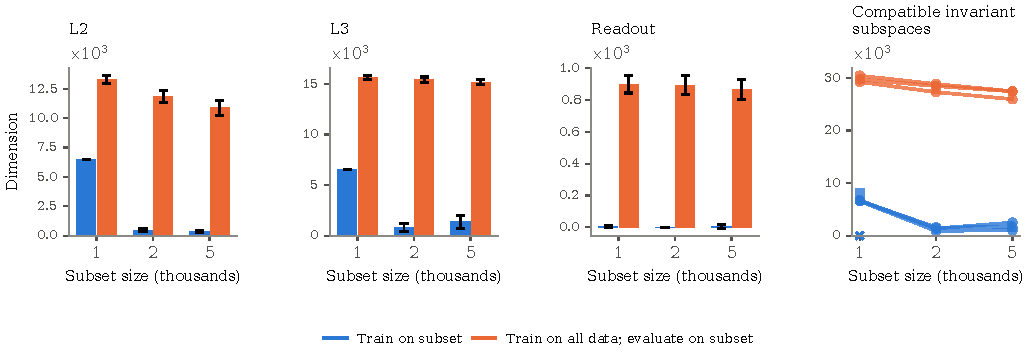
\includegraphics[width=6.156in]{data_dimensions_four.pdf}
\caption{Dimensions at epoch 500 versus subset size, width-128 ReLU MLPs. Colors distinguish subset-trained and full-data networks throughout. First three panels: total atomic dimensions, with seed means and sample-standard-deviation whiskers. Fourth: compatible invariant subspace dimensions, with one curve per seed; solid/circles denote bottom-up construction, dashed/squares top-down, and dotted/crosses the atomic sum. Zero means no validated direction, including a failed certificate. Unmeasured constructions have no point. L1 is fixed.}\label{fig:data-atomic}\label{fig:data-branches}
\end{figure}
\FloatBarrier
